% ju 23-Jul-21
\section*{Einleitung}

\emph{Sonderzeichen}  wie <<\& oder \%>> müssen mit einem Backslash \verb|\& oder \%| maskiert werden, 
damit sie von LaTeX nicht als Befehle missverstanden werden.


\emph{Website} \footnote{\url{https://golatex.de/wiki/Hauptseite}} \verb|\footnote{\url{https://golatex.de/wiki/Hauptseite}}| 


\clearpage
\subsection*{Stand der Forschung}

Während die traditionelle Latexproduktion bereits hinreichend erforscht ist (\autoref{fig:latex}) \\
\verb|(\autoref{fig:latex})|, bleibt das wissenschaftliche Verständnis elektronischer Verarbeitungsprozesse dieses 
vielseitigen Materials weiterhin lückenhaft. 


\begin{figure}[!ht]% hier: !ht
	\centering
	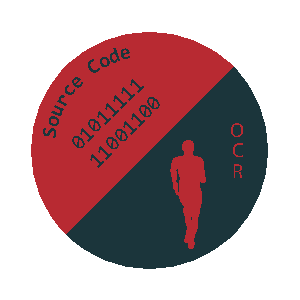
\includegraphics[width=0.25\textwidth]{images/Logo/logo.eps}
	\caption{Traditionelle Latexproduktion}\label{fig:latex}%
\end{figure}

\clearpage
\section*{Ausblick}

Daraus ergeben sich gemäß (\autoref{tab:schritte}) \verb|(\autoref{tab:schritte})| folgende nächste Schritte, 
deren sequenzielle Ausführung von essenzieller Bedeutung ist.

\begin{table}[!ht]% hier: !ht
	\centering
	\begin{tabular}{@{}cl@{}}% lcr
		\toprule
		\textbf{Nr.} & \textbf{Vorgehen} \\
		\midrule
		1 & Aktuellen Forschungsstand recherchieren \\
		2 & Methoden entwickeln \\
		3 & Schlussfolgerung aufstellen \\
		\bottomrule
	\end{tabular}
	\caption{Nächste Schritte}\label{tab:schritte}
\end{table}

